%%%%%%%%%%%%%%%%%%%%%%%%%%%%%%%%%%%%%%%%%%%%%%%%%%%%%%%%%%%%%%%%%%%%%%%%%%%%%%%%
%2345678901234567890123456789012345678901234567890123456789012345678901234567890
%        1         2         3         4         5         6         7         8
%\documentclass[twocolumn, journal]{IEEEtran}
\documentclass[onecolumn, journal]{IEEEtran}  % Comment this line out
                                                          % if you need a4paper
%\documentclass[letterpaper, 10pt, conference]{ieeeconf}      % Use this line for a4
                                                          % paper

\IEEEoverridecommandlockouts                              % This command is only
                                                          % needed if you want to
                                                          % use the \thanks command
\overrideIEEEmargins
% See the \addtolength command later in the file to balance the column lengths
% on the last page of the document
% The following packages can be found on http:\\www.ctan.org
\usepackage[utf8]{inputenc}
\usepackage{amsmath,bm}
\usepackage{amsfonts}
\usepackage{amssymb}
\usepackage{graphicx}
\usepackage{amsfonts}
\usepackage{hyperref}
\usepackage{caption}
\usepackage{subcaption}
\usepackage{algorithm}
\usepackage[noend]{algpseudocode}
%\usepackage{amsthm}
\usepackage{xcolor}
%\usepackage{subfig}
\usepackage{cite}
\usepackage[normalem]{ulem}
\DeclareMathOperator{\rk}{{rank}}
\DeclareMathOperator{\tr}{{trace}}
\DeclareMathOperator{\sgn}{{sgn}}
\DeclareMathOperator{\doc}{{doc}}
\newtheorem{definition}{Definition}
\newtheorem{Theorem}{Theorem}
%\numberwithin{Theorem}{section}
\newtheorem{Proposition}{Proposition}
\newtheorem{Lemma}{Lemma}
%\numberwithin{Lemma}{section}
\newtheorem{Problem}{Problem}
%\numberwithin{Problem}{section}
%\newtheorem*{Problem}{Problem}
\newtheorem{Corollary}{Corollary}
\newtheorem{Remark}{Remark}
\newtheorem{Assumption}{Assumption}
% draw graph pagkage
\usepackage{tikz}
	\usetikzlibrary{shadows,shapes,arrows}
	\tikzstyle{frame} = [draw, -latex]
	\tikzstyle{line} = [draw]
	\tikzstyle{line2} = [draw, dashdotted]
	\tikzstyle{line3} = [draw, dashed]
	\tikzstyle{line3UD} = [draw, dashed]
	\tikzstyle{place} = [circle, draw=black, fill=white, thick, inner sep=2pt, minimum size=1mm]
	\tikzstyle{place2} = [circle, draw=black, fill=black, thick, inner sep=2pt, minimum size=1mm]
	\tikzstyle{placeRed} = [circle, draw=red, fill=red, thick, inner sep=2pt, minimum size=1mm]
	\tikzstyle{vertex} = [circle, draw=black, fill=black, thick, inner sep=2pt, minimum size=1mm]
\usepackage{tkz-euclide}
\usepackage{multirow}

\newcommand{\m}[1]{\mathbf{#1}}
\newcommand{\mc}[1]{\mathcal{#1}}
\newcommand{\mb}[1]{\mathbb{#1}}
\newcommand{\abs}[1]{\lVert{#1} \rVert}
\newcommand\numberthis{\addtocounter{equation}{1}\tag{\theequation}}
\newcommand*{\eprf}{\hfill\ensuremath{\blacksquare}}%%%% Add for proof
\makeatletter
% Reinsert missing \algbackskip
\def\algbackskip{\hskip-\ALG@thistlm}
\makeatother
\usepackage[switch,pagewise]{lineno}
%\usepackage[switch,columnwise]{lineno}
% The following packages can be found on http:\\www.ctan.org
%\usepackage{graphics} % for pdf, bitmapped graphics files
%\usepackage{epsfig} % for postscript graphics files
%\usepackage{mathptmx} % assumes new font selection scheme installed
%\usepackage{times} % assumes new font selection scheme installed
%\usepackage{amsmath} % assumes amsmath package installed
%\usepackage{amssymb}  % assumes amsmath package installed
%\usepackage{setspace}}
\allowdisplaybreaks

\title{\LARGE \bf Distributed least square solution method to linear algebraic equations over multiagent networks}
\author{Viet Hoang Pham$^{1}$ and Hyo-Sung Ahn$^{1}$ 
\thanks{\small $^{1}$School of Mechanical Engineering, Gwangju Institute of Science and Technology, Gwangju, Korea. E-mails: {vietph@gist.ac.kr}; {hyosung@gist.ac.kr.}}
}

\begin{document}
%\doublespacing
%%%%%%%%%%%%%%%%%%%%%%%%%%%%%%%%%%%%%%%%%%%%%%%%%%%%%%%%%%%%%%%%%%%%%%%%
%\linenumbers
%\pagewiselinenumbers
\maketitle 
\thispagestyle{empty}
\pagestyle{empty}
%%%%%%%%%%%%%%%%%%%%%%%%%%%%%%%%%%%%%%%%%%%%%%%%%%%%%%%%%%%%%%%%%%%%%%%%%%%%%%%%%%%%%%%%%%
\begin{abstract}
%%%%%%%%%%%%%%%%%%%%%%%%%%%%%%%%%%%%%%%%%%%%%%%%%%%%%%%%%%%%%%%%%%%%%%%%%%%%%%%%%%%%%%%%%%
This paper designs a distributed least square solution method for a linear algebraic equation over a multiagent network. The coefficient matrix is divided into multiple blocks, and each agent only knows a subset of these blocks. The designed method is discrete-time and based on a proximal ADMM algorithm.
By applying the designed method, each agent can find its corresponding part in one least square solution of the considered linear algebraic equation while using only its information and communicating with its neighbors.
Numerical simulations verify the effectiveness of the designed method in MATLAB.
%%%%%%%%%%%%%%%%%%%%%%%%%%%%%%%%%%%%%%%%%%%%%%%%%%%%%%%%%%%%%%%%%%%%%%%%%%%%%%%%%%%%%%%%%%
\end{abstract}
%%%%%%%%%%%%%%%%%%%%%%%%%%%%%%%%%%%%%%%%%%%%%%%%%%%%%%%%%%%%%%%%%%%%%%%%%%%%%%%%%%%%%%%%%%
\section{Introduction}
%%%%%%%%%%%%%%%%%%%%%%%%%%%%%%%%%%%%%%%%%%%%%%%%%%%%%%%%%%%%%%%%%%%%%%%%%%%%%%%%%%%%%%%%%%
Multiagent system control and optimization have become popular in many applications. The reliance is due to the inherent complexity of large-scale problems and memory dispersion with the growth of big data. Depending on the communication network among agents, a multiagent system can have a hierarchical or distributed scheme. In a hierarchical setup, one master agent plays as a coordinator. This agent communicates with and/or assigns tasks to all others. In a distributed setup, agents work in parallel, and each agent can exchange information with only its neighbors. Because of the scalability and privacy protection requirements, distributed ones have become more desired recently.

Many fundamental problems in diverse engineering applications can be deduced into solving a linear algebraic equation $\textbf{H}\textbf{z} = \textbf{h}$ where $\textbf{H}$ and $\textbf{h}$ are coefficient matrix and vector. Various distributed methods have been developed to find the solution of $\textbf{H}\textbf{z} = \textbf{h}$ while each agent knows only a subset of rows in $\textbf{H}$ and $\textbf{h}$. The first approach considers constrained consensus problems \cite{ShaoshuaiMou2015, JiLiu2017, JiLiu2018, JiLiu2016}. By using an orthogonal projection of the kernel of the local coefficient matrix, the estimated solution of every agent always satisfies its linear equations. Distributed consensus schemes are exploited to drive estimated solutions of all agents to converge to an agreement. The methods in \cite{ShaoshuaiMou2015, JiLiu2017, JiLiu2018} are discrete-time while the one in \cite{JiLiu2016} is continuous-time. The convergence of these methods is guaranteed only if the considered linear algebraic equation has at least one exact solution.

Another approach considers the problem of solving the distributed linear algebraic equation as finding the optimal solution of a multiagent optimization problem. The local cost function in each agent is the total square error of its local linear equations, and the constraints are added to force the agreement for estimated solutions among neighboring agents. Various distributed optimization algorithms, such as subgradient-based methods \cite{BahmanGharesifard2014, GuannanQu2017}, ADMM \cite{BingshengHe2015, XinxinLi2015}, can be applied to solve the optimization problem. When the considered linear algebraic equation has one or several exact solutions, all agents can asymptotically determine one of such points \cite{PengWang2022}. If the exact solution does not exist, the final converged solution minimizes the total square errors of linear equations \cite{XuanWang2019, YangLiu2019, TaoYang2020}.

This paper considers the problem of finding a least square solution of a distributed linear algebraic equation $\textbf{H}\textbf{z} = \textbf{h}$ over a network of agents.
In which not only the rows but also the columns of $\textbf{H}$ and $\textbf{h}$ are distributed among individual agents. Let the matrix $\textbf{H}$ be divided into multiple blocks. Each agent only knows a subset of the divided blocks.
Different from \cite{XuanWang2020}, we do not require an aggregator to collect information from agents corresponding to the same rows. Instead, we introduce some virtual variables to transform the coupling linear equations, whose data are dispensed across multiple agents, into local constraints of individual agents combining coupling constraints among neighboring agents. Consequently, we obtain a distributed optimization problem whose optimal solution is one least square solution of the considered linear algebraic equation. Then we apply a proximal ADMM algorithm \cite{BingshengHe2015, XinxinLi2015} to design a distributed method to find the optimal solution of the obtained distributed optimization problem.
Since the designed method is discrete-time, the asymptotic convergence of the ADMM-based solution method implies the exponential convergence of the estimated solution to the optimal one.
Our designed method has no requirements for step-size selection or initial point setup. In addition, each agent is required to use only its information and communicate with its neighbors.

The remainder of the paper is organized as follows. Section II provides some preliminaries for the analysis in later sections. In Section III, we describe the setup of the distributed linear algebraic equation and introduce the problem of finding the least square solution in an optimization based approach. Then we formulate a distributed optimization problem whose optimal solution can be used to determine the least square solution of the considered linear algebraic equation in Section IV. In this section, we apply a proximal ADMM algorithm \cite{BingshengHe2015, XinxinLi2015} to design a distributed solution method for the formulated optimization problem. Numerical simulations are provided in Section V to illustrate the effectiveness of the proposed method. Section VI concludes this paper.
%%%%%%%%%%%%%%%%%%%%%%%%%%%%%%%%%%%%%%%%%%%%%%%%%%%%%%%%%%%%%%%%%%%%%%%%%%%%%%%%%%%%%%%%%%
%%%%%%%%%%%%%%%%%%%%%%%%%%%%%%%%%%%%%%%%%%%%%%%%%%%%%%%%%%%%%%%%%%%%%%%%%%%%%%%%%%%%%%%%%%
\section{Preliminaries}
%%%%%%%%%%%%%%%%%%%%%%%%%%%%%%%%%%%%%%%%%%%%%%%%%%%%%%%%%%%%%%%%%%%%%%%%%%%%%%%%%%%%%%%%%%
\subsection{Notations}
%%%%%%%%%%%%%%%%%%%%%%%%%%%%%%%%%%%%%%%%%%%%%%%%%%%%%%%%%%%%%%%%%%%%%%%%%%%%%%%%%%%%%%%%%%
We use $\mathbb{R}, \mathbb{R}^n$ and $\mathbb{R}^{m \times n}$ to denote respectively the set of real numbers, the set of $n$-dimension real vectors, and the set of real matrices having $m$ rows and $n$ columns.
Denote by $\textbf{1}_n$ and $\textbf{0}_n$ the vectors in $\mathbb{R}^{n}$ whose all elements are $1$ and $0$, respectively.
Let $\textbf{I}_n$ be the identity matrix in $\mathbb{R}^{n \times n}$ and $\textbf{0}_{m \times n}$ be the zero matrix in $\mathbb{R}^{m \times n}$. When the dimensions are clear, the subscripts of the matrices $\textbf{I}_n, \textbf{0}_{m \times n}$ and the vector $\textbf{0}_n$ can be removed.
$\textbf{H} \succ 0$ ($\succeq 0$) means $\textbf{H}$ is a positive (semi-)definite matrix.

Denote by $\textbf{H}^T$ the transpose matrix of $\textbf{H}$.
Define $||\textbf{x}||_{\textbf{H}}^2 = \textbf{x}^T\textbf{H}\textbf{x}$. When $\textbf{H} = \textbf{I}$, we write $||\textbf{x}||^2$ for simplicity. If $x$ is a scalar, we write $|x| = ||x||$.

A list corresponds to an ordered set of elements and elements in a list can be duplicated.
For a list $\mathcal{A}$, define $\mathbb{S}(\mathcal{A})$ as the set obtained from the the list $\mathcal{A}$ by considering duplicated elements in $\mathcal{A}$ as one element. Let $|\mathbb{S}(\mathcal{A})|$ denote its cardinality. Consider two set $\mathbb{S}_1$ and $\mathbb{S}_2$, the difference of these two sets is denoted by $\mathbb{S}_1-\mathbb{S}_2 = \{a \in \mathbb{S}_1: a \notin \mathbb{S}_1\}$.

Let $\mathcal{A} = \left\{\textbf{h}_1, \textbf{h}_2, \dots, \textbf{h}_m\right\}$ be the list of $m$ vectors, we define the column vector \[\textrm{col } \mathcal{A} = \textrm{col} \left\{\textbf{h}_1, \textbf{h}_2, \dots, \textbf{h}_m\right\} = \left[\textbf{h}_1^T, \textbf{h}_2^T, \dots, \textbf{h}_m^T\right]^T.\]
For a list of matrices, $\mathcal{A} = \left\{\textbf{H}_1, \textbf{H}_2, \dots, \textbf{H}_m\right\}$, we use $\textrm{blkdiag }\mathcal{A}$ to denote the block-diagonal matrix whose main block are matrices in the list $\mathcal{A}$, and use $\textrm{blkrow }\mathcal{A}$ and $\textrm{blkcol }\mathcal{A}$ to denote the following two matrices respectively:
\[\textrm{blkrow}\left\{\textbf{H}_1, \textbf{H}_2, \dots, \textbf{H}_m\right\} = \left[\begin{matrix}\textbf{H}_1 & \textbf{H}_2 & \cdots & \textbf{H}_m\end{matrix}\right],\]
\[\textrm{blkcol}\left\{\textbf{H}_1, \textbf{H}_2, \dots, \textbf{H}_m\right\} = \left[\begin{matrix}\textbf{H}_1^T & \textbf{H}_2^T & \cdots & \textbf{H}_m^T\end{matrix}\right]^T.\]
%%%%%%%%%%%%%%%%%%%%%%%%%%%%%%%%%%%%%%%%%%%%%%%%%%%%%%%%%%%%%%%%%%%%%%%%%%%%%%%%%%%%%%%%%%
\subsection{Graph theory}
%%%%%%%%%%%%%%%%%%%%%%%%%%%%%%%%%%%%%%%%%%%%%%%%%%%%%%%%%%%%%%%%%%%%%%%%%%%%%%%%%%%%%%%%%%
Let $\mathcal{G} = (\mathcal{V}, \mathcal{E})$ be a graph where $\mathcal{V} = \{1, 2, \dots\}$ is the node set and $\mathcal{E} \subset \mathcal{V} \times \mathcal{V}$ is the edge set.
The graph $\mathcal{G}$ is undirected if $(i,j) \in \mathcal{E}$ implies $(j,i) \in \mathcal{E}$ for every pair of nodes $i,j \in \mathcal{V}$.
The graph $\mathcal{G}$ is a connected graph if there is a path from $i$ to $j$ for any pair $i,j \in \mathcal{V}$, which means there is a sequence of edges $(i_1,i_2), (i_2,i_3), \dots, (i_{k-1},i_k)$ such that $i_1 = i, i_k = j$ and $i_m \in \mathcal{V}, (i_{m-1},i_m) \in \mathcal{E}, \forall 2 \le m \le k$.

For a node subset $\tilde{\mathcal{V}} \subset \mathcal{V}$, the subgraph induced by $\tilde{\mathcal{V}}$ is defined as $(\tilde{\mathcal{V}}, \tilde{\mathcal{E}})$ where $\tilde{\mathcal{E}} = \{(i,j) \in \mathcal{E}: i,j \in \tilde{\mathcal{V}}\}$.
%%%%%%%%%%%%%%%%%%%%%%%%%%%%%%%%%%%%%%%%%%%%%%%%%%%%%%%%%%%%%%%%%%%%%%%%%%%%%%%%
\subsection{Proximal ADMM Algorithm}
%%%%%%%%%%%%%%%%%%%%%%%%%%%%%%%%%%%%%%%%%%%%%%%%%%%%%%%%%%%%%%%%%%%%%%%%%%%%%%%%%%%%%%%%%%
Consider the following convex optimization problem
\begin{equation}\label{eq_ADMMproblem}
\min\limits_{\textbf{x} \in \mathcal{X}, \textbf{y} \in \mathcal{Y}} \textrm{ }\Psi_x(\textbf{x}) + \Psi_y(\textbf{y}) \textrm{ s.t. } \textbf{F}_x\textbf{x} + \textbf{F}_y\textbf{y} = \textbf{f}.
\end{equation}
where $\Psi_x(\textbf{x}), \Psi_y(\textbf{y})$ are convex functions, $\mathcal{X}, \mathcal{Y}$ are convex sets, $\textbf{F}_x, \textbf{F}_y$ and $\textbf{f}$ are known matrices and vector.
Define the augmented Lagrangian function of the problem \eqref{eq_ADMMproblem} as \[\mathcal{L}_{\rho}(\textbf{x},\textbf{y},\boldsymbol{\lambda}) = \Psi_x(\textbf{x}) + \Psi_y(\textbf{y}) + \frac{\rho}{2}\Bigl|\Bigl|\textbf{F}_x\textbf{x} + \textbf{F}_y\textbf{y} - \textbf{f} - \frac{1}{\rho}\boldsymbol{\lambda}\Bigr|\Bigr|^2\] where $\boldsymbol{\lambda}$ is the dual variable associated with the equality constraint and $\rho > 0$ is a positive penalty parameter.
The proximal ADMM scheme for solving \eqref{eq_ADMMproblem} is given by the iteration update \eqref{eq_ADMM} as follows.
\begin{subequations}\label{eq_ADMM}
\begin{align}
&\textbf{x}(s+1) = \arg\min\limits_{\textbf{x} \in \mathcal{X}} \Bigl\{\mathcal{L}_{\rho}(\textbf{x},\textbf{y}(s),\boldsymbol{\lambda}(s)) + \frac{1}{2}\left|\left|\textbf{x} - \textbf{x}(s)\right|\right|_{\textbf{G}}^2 \Bigr\},\\
&\textbf{y}(s+1) = \arg\min\limits_{\textbf{y} \in \mathcal{Y}} \mathcal{L}_{\rho}(\textbf{x}(s+1),\textbf{y},\boldsymbol{\lambda}(s)),\\
&\boldsymbol{\lambda}(s+1) = \boldsymbol{\lambda}(s) - \rho \Bigl(\textbf{F}_x\textbf{x}(s+1) + \textbf{F}_y\textbf{y}(s+1) - \textbf{f}\Bigr),
\end{align}
\end{subequations}
where $\textbf{G}$ is a symmetric and positive semidefinite matrix and the initial point $(\textbf{x}(0), \textbf{y}(0), \boldsymbol{\lambda}(0))$ can be chosen arbitrarily such that $\textbf{x}(0) \in \mathcal{X}, \textbf{y}(0) \in \mathcal{Y}$.
The following theorem summarizes the results in \cite{XinxinLi2015} for the convergence of the proximal ADMM algorithm \eqref{eq_ADMM}.
\begin{Theorem}\label{th_ADMM}
Let $\boldsymbol{\Theta} = blkdiag\left\{ \textbf{G}, \rho\textbf{F}_y^T\textbf{F}_y, \frac{1}{\rho}\textbf{I} \right\}$ and $\textbf{w}(s) = [\textbf{x}(s)^T, \textbf{y}(s)^T, \boldsymbol{\lambda}(s)^T]^T$. Then we have
\begin{enumerate}
\item $||\textbf{w}(s) - \textbf{w}(s+1)||_{\boldsymbol{\Theta}}^2 = o\left(\frac{1}{s}\right)$
\item $|| \textbf{F}_x\textbf{x}(s) + \textbf{F}_y\textbf{y}(s) - \textbf{f}|| = o\left(\frac{1}{\sqrt{s}}\right)$
\item $|\psi_x(\textbf{x}(s)) + \psi_y(\textbf{y}(s)) - \psi^{opt}| = o\left(\frac{1}{\sqrt{s}}\right)$ where $\psi^{opt}$ is the optimal cost value of the problem \eqref{eq_ADMMproblem}.
\end{enumerate}
\end{Theorem}
The item 1) and 2) \& 3) of Theorem \ref{th_ADMM} are corresponding to Theorem 5.2 and Corollary 5.1 in \cite{XinxinLi2015}, respectively.
%%%%%%%%%%%%%%%%%%%%%%%%%%%%%%%%%%%%%%%%%%%%%%%%%%%%%%%%%%%%%%%%%%%%%%%%%%%%%%%%%%%%%%%%%%
\subsection{Quadratic program with equality constraint}\label{subQP}
%%%%%%%%%%%%%%%%%%%%%%%%%%%%%%%%%%%%%%%%%%%%%%%%%%%%%%%%%%%%%%%%%%%%%%%%%%%%%%%%%%%%%%%%%%
Consider a quadratic program with only equality constraints as \eqref{eq_QP}.
\begin{equation}\label{eq_QP}
\min\limits_{\textbf{H}\textbf{x} = \textbf{h}} \left(\frac{1}{2} \textbf{x}^T\textbf{Q}\textbf{x} + \textbf{q}^T\textbf{x}\right).
\end{equation}
where $\textbf{Q} \succ 0$ and $\textbf{H}$ is a full row rank matrix.
Let $\textbf{x}^{opt}$ be the optimal solution of \eqref{eq_QP}. Since the Karuhs-Kuhn-Tucker conditions is necessary and sufficient conditions for the optimality, $\textbf{x}^{opt}$ is the solution of the linear equation \eqref{eq_temp1OptimizationConditions} as follows.
\begin{subequations}\label{eq_temp1OptimizationConditions}
\begin{align}
\textbf{Q}\textbf{x} + \textbf{q} - \textbf{H}^T \boldsymbol{\mu} &= \textbf{0}\\
\textbf{H}\textbf{x} &= \textbf{h}
\end{align}
\end{subequations}
where $\boldsymbol{\mu}$ is the dual variable.
By solving (\ref{eq_temp1OptimizationConditions}a), we obtain
\begin{align}
\textbf{x}^{opt} =& \textbf{Q}^{-1}\left(\textbf{H}^T\left(\textbf{H}\textbf{Q}^{-1}\textbf{H}^T\right)^{-1}\textbf{H}\textbf{Q}^{-1} - \textbf{I}\right)\textbf{q} + \textbf{Q}^{-1}\textbf{H}^T\left(\textbf{H}\textbf{Q}^{-1}\textbf{H}^T\right)^{-1}\textbf{h}. \label{eq_updatelaw_temp_a}
\end{align}
%%%%%%%%%%%%%%%%%%%%%%%%%%%%%%%%%%%%%%%%%%%%%%%%%%%%%%%%%%%%%%%%%%%%%%%%%%%%%%%%%%%%%%%%%%
%%%%%%%%%%%%%%%%%%%%%%%%%%%%%%%%%%%%%%%%%%%%%%%%%%%%%%%%%%%%%%%%%%%%%%%%%%%%%%%%%%%%%%%%%%
\section{Problem statement}
%%%%%%%%%%%%%%%%%%%%%%%%%%%%%%%%%%%%%%%%%%%%%%%%%%%%%%%%%%%%%%%%%%%%%%%%%%%%%%%%%%%%%%%%%%
\subsection{Distributed problem setup}
%%%%%%%%%%%%%%%%%%%%%%%%%%%%%%%%%%%%%%%%%%%%%%%%%%%%%%%%%%%%%%%%%%%%%%%%%%%%%%%%%%%%%%%%%%
Consider a linear algebraic equation
\begin{equation}\label{eq_LE}
\textbf{H}\textbf{z} = \textbf{h}
\end{equation}
where $\textbf{z}$ is the unknown vector, $\textbf{H}$ and $\textbf{h}$ are coefficients matrix and vector, respectively.
In general, the linear algebraic equation \eqref{eq_LE} can have one or more least square solutions.
Let $\textbf{z}^{opt}$ be one least square solution to \eqref{eq_LE}. Then we have
\begin{equation}\label{eq_LE_solution}
\textbf{z}^{opt} = \arg\min_{\textbf{z}} \frac{1}{2}\bigl|\bigl|\textbf{H}\textbf{z} - \textbf{h}\bigr|\bigr|^2.
\end{equation}
Define $\Phi^{opt} = ||\textbf{H}\textbf{z}^{opt} - \textbf{h}||^2$.
We have $\Phi^{opt} = 0$ if the linear algebraic equation \eqref{eq_LE} has at least one exact solution. If $\textbf{H}$ is a full column rank matrix, we have $\textbf{z}^{opt} = (\textbf{H}^T\textbf{H})^{-1}\textbf{H}^T\textbf{h}$ is unique and $\Phi^{opt} = \textbf{h}^T\textbf{h} - \frac{1}{2}\textbf{h}^T\textbf{H}(\textbf{H}^T\textbf{H})^{-1}\textbf{H}^T\textbf{h}$.

Suppose that the coefficient matrix $\textbf{H}$ can be subdivided into the following form:
\begin{equation}\label{eq_LE_partitions}
\textbf{H} = \left[\begin{matrix}
\textbf{H}_{11} & \textbf{H}_{12} & \cdots & \textbf{H}_{1L}\\
\textbf{H}_{21} & \textbf{H}_{22} & \cdots & \textbf{H}_{2L}\\
\vdots & \vdots & \ddots & \vdots\\
\textbf{H}_{K1} & \textbf{H}_{K2} & \cdots & \textbf{H}_{KL}
\end{matrix}\right].
\end{equation}
That means the coefficient matrix $\textbf{H}$ is divided into $KL$ blocks corresponding to $K$ row and $L$ column partitions.
In this paper, we focus on the problem of determing one least square solution to the linear algebraic equation \eqref{eq_LE} when each nonzero block $\textbf{H}_{kl}$ in \eqref{eq_LE_partitions} is known by only one agent in a network of $N$ agents. The information of zero blocks, i.e., $\textbf{H}_{kl} = \textbf{0}$ for some $k,l$, is not stored in any agents.
 
For each row partition $k$, $1 \le k \le K$, of the matrix $\textbf{H}$, we define $\mathcal{R}_k$ as the index list of agents who knows blocks in the set $\{\textbf{H}_{k1}, \textbf{H}_{k2}, \dots, \textbf{H}_{kL}\}$. Similarly, we define $\mathcal{C}^l$ as the set of agents who knows blocks in the set $\{\textbf{H}_{1l}, \textbf{H}_{2l}, \dots, \textbf{H}_{Kl}\}$ for all $1 \le l \le L$.
As $\mathcal{R}_k$ and $\mathcal{C}^l$ are lists, they can contain duplicated indexes. For the zero block, i.e., $\textbf{H}_{kl} = \textbf{0}$ for some $k,l$, we use index $0$ in the corresponding lists $\mathcal{R}_k$ and $\mathcal{C}^l$.

To illustrate the definition of index lists, we consider an example as shown in Fig. \ref{fig_example}.
\begin{figure}[htb]
\centering
\scalebox{0.95}{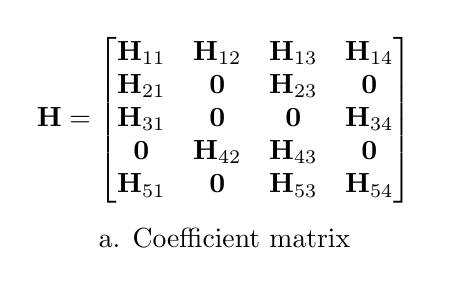
\begin{tikzpicture}
\node[] at (0,1.5) {$\textbf{H} = \left[\begin{matrix}
\textbf{H}_{11} & \textbf{H}_{12} & \textbf{H}_{13} & \textbf{H}_{14}\\
\textbf{H}_{21} & \textbf{0} & \textbf{H}_{23} & \textbf{0}\\
\textbf{H}_{31} & \textbf{0} & \textbf{0} & \textbf{H}_{34}\\
\textbf{0} & \textbf{H}_{42} & \textbf{H}_{43} & \textbf{0}\\
\textbf{H}_{51} & \textbf{0} & \textbf{H}_{53} & \textbf{H}_{54}
\end{matrix}\right]$};
\node[] at (0,0) {a. Coefficient matrix};
\end{tikzpicture}}
\scalebox{0.95}{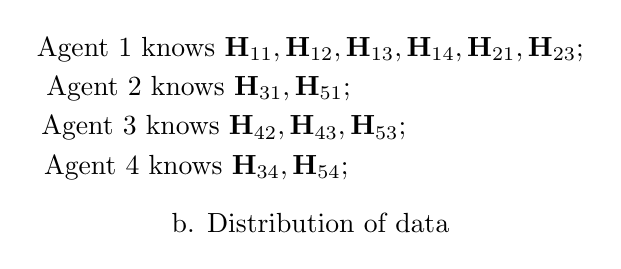
\begin{tikzpicture}
\node[] at (0,2.5) {Agent $1$ knows $\textbf{H}_{11}, \textbf{H}_{12}, \textbf{H}_{13}, \textbf{H}_{14}, \textbf{H}_{21}, \textbf{H}_{23}$;};
\node[] at (-1.42,2) {Agent $2$ knows $\textbf{H}_{31}, \textbf{H}_{51}$;};
\node[] at (-1.1,1.5) {Agent $3$ knows $\textbf{H}_{42}, \textbf{H}_{43}, \textbf{H}_{53}$;};
\node[] at (-1.45,1) {Agent $4$ knows $\textbf{H}_{34}, \textbf{H}_{54}$;};
\node[] at (0,0.3) {b. Distribution of data};
\end{tikzpicture}}
\caption{Example of distributed linear algebraic equation over a network of $4$ agents.}\label{fig_example}
\end{figure}
We have $\mathcal{R}_1 = \{1, 1, 1, 1\}$, $\mathcal{R}_2 = \{1, 0, 1, 0\}$, $\mathcal{R}_3 = \{2, 0, 0, 4\}$, $\mathcal{R}_4 = \{0, 3, 3, 0\}$, $\mathcal{R}_5 = \{2, 0, 0, 4\}$ and $\mathcal{C}^1 = \{1, 1, 2, 0, 2\}$, $\mathcal{C}^2 = \{1, 0, 0, 3, 0\}$, $\mathcal{C}^3 = \{1, 1, 0, 3, 0\}$, $\mathcal{C}^4 = \{1, 0, 4, 0, 4\}$.
The sets corresponding to these lists are: $\mathbb{S}(\mathcal{R}_1) = \{1\}$, $\mathbb{S}(\mathcal{R}_1) = \{1, 0\}$, $\mathbb{S}(\mathcal{R}_3) = \{2, 0, 4\}$, $\mathbb{S}(\mathcal{R}_4) = \{0, 3\}$, $\mathbb{S}(\mathcal{R}_5) = \{2, 0, 3, 4\}$ and $\mathbb{S}(\mathcal{C}^1) = \{1, 0, 2\}$, $\mathbb{S}(\mathcal{C}^1) = \{1, 0, 3\}$, $\mathbb{S}(\mathcal{C}^1) = \{1, 0, 3\}$, $\mathbb{S}(\mathcal{C}^1) = \{1, 0, 4\}$.

Since we can obtain an equivalent linear algebraic equation to \eqref{eq_LE} if we exchange rows in the matrix $\textbf{H}$ and the vector $\textbf{h}$. So, the rows in $\textbf{H}$ can be interchanged such that the ones dispensed across the same set of agents are grouped in the same row partition.
Without loss of generality, we assume that $\mathcal{R}_k \neq \mathcal{R}_{k'}$ if $k \neq k'$ for all $ 1 \le k,k' \le K$.
According to the partition of $\textbf{H}$, the unknown vector $\textbf{z}$ and the coefficient vector $\textbf{h}$ can be partitioned as:
\[\textbf{z} = \textrm{col}\{\textbf{z}_{1}, \textbf{z}_{2}, \dots, \textbf{z}_{L}\},
\textbf{h} = \textrm{col}\{\textbf{h}_{1}, \textbf{h}_{2}, \dots, \textbf{h}_{K}\}.\]
To consider the distributed linear algebraic equation \eqref{eq_LE} in a distributed setup, we assume that each agent $i$ in the set $\mathbb{S}(\mathcal{R}_k)$ knows a vector $\textbf{h}_{i,k}$ such that
\begin{equation}\label{eq_aspt_coupled_equations}
\sum_{i \in \mathbb{S}(\mathcal{R}_k)} \textbf{h}_{i,k} = \textbf{h}_k, \forall 1 \le k \le K.
\end{equation}
%%%%%%%%%%%%%%%%%%%%%%%%%%%%%%%%%%%%%%%%%%%%%%%%%%%%%%%%%%%%%%%%%%%%%%%%%%%%%%%%%%%%%%%%%%
\subsection{Communication graph}
%%%%%%%%%%%%%%%%%%%%%%%%%%%%%%%%%%%%%%%%%%%%%%%%%%%%%%%%%%%%%%%%%%%%%%%%%%%%%%%%%%%%%%%%%%
In this paper, we use an undirected graph $\mathcal{G} = (\mathcal{V}, \mathcal{E})$ to illustrate the communication among a network of multiple agents.
Each node $i \in \mathcal{V} = \{1, 2, \dots, N\}$ corresponds to an agent while an edge $(i,j) \in \mathcal{E}$ represents that the agent $i$ can exchange information with the agent $j$.
The set of neighbors of the agent $i \in \mathcal{V}$ is denoted by $\mathcal{N}_i = \left\{j \in \mathcal{V}: (i,j) \in \mathcal{E}\right\}$.
For each row partition $k$, where $1 \le k \le K$, we have $\mathbb{S}(\mathcal{R}_k) \subset \mathcal{V}$ is a subset of nodes. We define $\mathcal{G}_{k} = (\mathbb{S}(\mathcal{R}_k), \mathcal{E}_{k})$ as the subgraph induced by the node set $\mathbb{S}(\mathcal{R}_k)$.
Similarly, we define $\mathcal{G}^{l} = (\mathbb{S}(\mathcal{C}^{l}), \mathcal{E}^{l})$ for each column partition $l$, where $1 \le l \le L$.

The following assumption is necessary.
\begin{Assumption}\label{aspt_topology}
The communication graph satisfies that
\begin{enumerate}
\item $\mathcal{G}_{k}$ is a connected graph for all $1 \le k \le K,$
\item $\mathcal{G}^{l}$ is a connected graph for all $1 \le l \le L$.
\end{enumerate}
\end{Assumption}
If $i \in \mathcal{C}^l$, the agent $i$ contains the information corresponding to the unknown part $\textbf{z}_l$, i.e., one or some nonzero blocks $\textbf{H}_{kl}$ where $1 \le k \le K$. So, the agent $i$ needs to estimate the unknown part $\textbf{z}_l$. The first item in Assumption \ref{aspt_topology} is to allow agents in the set $\mathbb{S}(\mathcal{C}^{l})$ can cooperatively achieve an agreement on the estimated solutions of $\textbf{z}_l$.
When $i \in \mathbb{S}(\mathcal{R}_k)$, the agent $i$ takes part in the linear equations corresponding to the row partition $k$.
In general, there are some row partitions $1 \le k \le K$ where $\mathbb{S}(\mathcal{R}_k) \neq \mathcal{N}_i$ for all $i \in \mathbb{S}(\mathcal{R}_k)$. Since communication is only available between two neighboring agents, it is difficult for one agent to collect complete information about the linear equations corresponding to these row partitions. The second item in Assumption \ref{aspt_topology} facilitates a transformation of these linear equations into local linear equations of individual agents combining coupling constraints among neighboring agents, as shown later in Subsection IV-A.
%%%%%%%%%%%%%%%%%%%%%%%%%%%%%%%%%%%%%%%%%%%%%%%%%%%%%%%%%%%%%%%%%%%%%%%%%%%%%%%%%%%%%%%%%%
\subsection{Problem statement}
%%%%%%%%%%%%%%%%%%%%%%%%%%%%%%%%%%%%%%%%%%%%%%%%%%%%%%%%%%%%%%%%%%%%%%%%%%%%%%%%%%%%%%%%%%
Let $\bar{\textbf{z}}_i = \textrm{col}\{\textbf{z}_l: i \in \mathbb{S}(\mathcal{C}^l)\}$ be the local variable of the agent $i \in \mathcal{V}$. For each neighboring agent $j \in \mathcal{N}_i$, define the matrix $\textbf{P}_{ij}$ such that $\textbf{P}_{ij}\bar{\textbf{z}}_i = \textrm{col}\{\textbf{z}_l: i,j \in \mathbb{S}(\mathcal{C}^l)\}$ corresponding to common variables of two agents $i$ and $j$. So, we have
\begin{equation}\label{eq_coupling_commonvariable}
\textbf{P}_{ij}\bar{\textbf{z}}_i = \textbf{P}_{ji}\bar{\textbf{z}}_j, \forall (i,j) \in \mathcal{E}.
\end{equation}
Consider a row partition $k$ where there is only one agent $i$ in the list $\mathcal{R}_k$. That means the set $\mathbb{S}(\mathcal{R}_k) = \{i\}$ or $\mathbb{S}(\mathcal{R}_k) = \{i,0\}$. In both cases, we have $\mathbb{S}(\mathcal{R}_k)-\{i,0\} = \emptyset$. Under the assumption of the equation \eqref{eq_aspt_coupled_equations}, the agent $i$ knows the vector $\textbf{h}_k$. The linear equations corresponding to this row partition, i.e, $\left[\begin{matrix} \textbf{H}_{k1}, \textbf{H}_{k2}, \dots, \textbf{H}_{kL} \end{matrix}\right]\textbf{z} = \textbf{h}_k$, can be rewritten as a local equation of the agent $i$ as \eqref{eq_local_equation_full}.
\begin{equation}\label{eq_local_equation_full}
\textbf{A}_i\bar{\textbf{z}}_i = \textbf{a}_i
\end{equation}
where $\textbf{A}_i$ is derived from the matrix $\textrm{blkcol}\{\textrm{blkrow}\{\textbf{H}_{kl} \neq \textbf{0}: l = 1, 2, \dots, L\}: \mathbb{S}(\mathcal{R}_k)-\{i,0\} = \emptyset\}$ removing zero columns and $\textbf{a}_i = \textbf{h}_k$.

Define by $\mathbb{B} = \{\epsilon_1, \epsilon_2, \dots, \epsilon_M\}$ the set of indexes of row partition $\epsilon_k$ where the list $\mathcal{R}_{\epsilon_k}$ contains of two or more agents. Let $\textbf{B}_{i,\epsilon_k}$ be the matrix constructed by blocks in the set $\{\textbf{H}_{\epsilon_kl}: i \in \mathbb{S}(\mathcal{R}_{\epsilon_k}) \cap \mathbb{S}(\mathcal{C}^l\})$ and zero matrices such that
\[\textbf{B}_{i,\epsilon_k}\bar{\textbf{z}}_i = \sum_{i \in \mathbb{S}(\mathcal{R}_{\epsilon_k}) \cap \mathbb{S}(\mathcal{C}^l\})}\textbf{H}_{\epsilon_kl}\textbf{z}_l.\]
The linear equations corresponding to the row partition $\epsilon_k \in \mathbb{B}$ can be rewritten as the coupling linear equation \eqref{eq_coupling_equation}.
\begin{equation}\label{eq_coupling_equation}
\sum_{i \in \mathbb{S}(\mathcal{R}_{\epsilon_k})} \textbf{B}_{i,\epsilon_k}\bar{\textbf{z}}_i = \sum_{i \in \mathbb{S}(\mathcal{R}_{\epsilon_k})} \textbf{b}_{i,\epsilon_k}, \forall \epsilon_k \in \mathbb{B}.
\end{equation}
We define by $\mathcal{B}_i = \{\epsilon_k \in \mathbb{B}: i \in \mathbb{S}(\mathcal{R}_{\epsilon_k})\}$ for each agent $i \in \mathcal{V}$.
Let $\textbf{u}_{\epsilon_k}$ be the error of the coupling equations in the row partition $\epsilon_k \in \mathbb{B}$, i.e.,
\begin{equation}\label{eq_LE_temp}
\textbf{u}_{\epsilon_k} = \sum_{i \in \mathbb{S}(\mathcal{R}_{\epsilon_k})} \left(\textbf{B}_{i,\epsilon_k}\bar{\textbf{z}}_i - \textbf{b}_{i,\epsilon_k}\right), \forall \epsilon_k \in \mathbb{B}.
\end{equation}
Consider the following optimization problem
\begin{equation}\label{eq_LE_optimizationproblem}
\min\limits_{\bar{\textbf{z}}_i, \textbf{u}_{\epsilon_k}} \frac{1}{2}\left(\sum_{i \in \mathcal{V}}||\textbf{A}_i\bar{\textbf{z}}_i - \textbf{a}_i||^2 + \sum_{\epsilon_k \in \mathcal{B}}||\textbf{u}_{\epsilon_k}||^2\right)
\textrm{ s.t. } \eqref{eq_coupling_commonvariable}, \eqref{eq_LE_temp}.
\end{equation}
It is clear that $\Phi^{opt} = ||\textbf{H}\textbf{z}^{opt} - \textbf{h}||^2$ is also the optimal cost function value of the problem \eqref{eq_LE_optimizationproblem} and from the optimal solution of \eqref{eq_LE_optimizationproblem} can be used to determine one least square solution \eqref{eq_LE_solution} of the linear algebraic equation \eqref{eq_LE}.
Thus we have the main problem of this paper as follows.
\begin{Problem}
Assume that the communication graph of the considered multiagent network satisfies Assumption \ref{aspt_topology}.
Design a distributed method for each agent to find its corresponding parts in one optimal solution of the constrained optimization problem \eqref{eq_LE_optimizationproblem} when using only its own information and exchanging information with other agents in the neighboring set $\mathcal{N}_i$.
\end{Problem}
We remark here that $\textbf{A}_i, \textbf{B}_{i,\epsilon_k}, \forall \epsilon_k \in \mathcal{B}_i,$ and $\textbf{a}_i, \textbf{b}_{i,\epsilon_k}, \forall \epsilon_k \in \mathcal{B}_i,$ are known by only the agent $i \in \mathcal{V}$.
%%%%%%%%%%%%%%%%%%%%%%%%%%%%%%%%%%%%%%%%%%%%%%%%%%%%%%%%%%%%%%%%%%%%%%%%%%%%%%%%%%%%%%%%%%
%%%%%%%%%%%%%%%%%%%%%%%%%%%%%%%%%%%%%%%%%%%%%%%%%%%%%%%%%%%%%%%%%%%%%%%%%%%%%%%%%%%%%%%%%%
\section{Distributed optimization approach}
%%%%%%%%%%%%%%%%%%%%%%%%%%%%%%%%%%%%%%%%%%%%%%%%%%%%%%%%%%%%%%%%%%%%%%%%%%%%%%%%%%%%%%%%%%
\subsection{Distributed optimization problem formulation}
%%%%%%%%%%%%%%%%%%%%%%%%%%%%%%%%%%%%%%%%%%%%%%%%%%%%%%%%%%%%%%%%%%%%%%%%%%%%%%%%%%%%%%%%%%
Consider the coupling subsystem of linear equations \eqref{eq_LE_temp} under the Assumption \ref{aspt_topology}, we have the following result:
\begin{Lemma}\label{lm_viratual}
For every $\epsilon_k \in \mathcal{B}$, there exist vectors $\textbf{u}_{\epsilon_k}$ and $\bar{\textbf{z}}_{\epsilon_k} = \textrm{col}\{\bar{\textbf{z}}_i: i \in \mathbb{S}(\mathcal{R}_{\epsilon_k})\}$ satisfying \eqref{eq_LE_temp} if and only if there exists $\textbf{v}_{\epsilon_k} = \textrm{col}\{\textbf{v}_{ij, \epsilon_k}: i,j \in \mathbb{S}(\mathcal{R}_{\epsilon_k})\}$ such that
\begin{equation}\label{eq_LE_virtual_var}
\frac{1}{|\mathbb{S}(\mathcal{R}_{\epsilon_k})|}\textbf{u}_{\epsilon_k} = \textbf{B}_{i,\epsilon_k}\bar{\textbf{z}}_i - \textbf{b}_{i,\epsilon_k} + \sum_{j \in \mathcal{N}_{i,\epsilon_k}} \left(\textbf{v}_{ij, \epsilon_k} - \textbf{v}_{ji, \epsilon_k}\right),
\end{equation}
for all $i \in \mathcal{R}_{\epsilon_k}$ where $\mathcal{N}_{i,\epsilon_k} \equiv \mathcal{N}_i \cap \mathbb{S}(\mathcal{R}_{\epsilon_k})$
\end{Lemma}
\begin{proof}
Suppose that \eqref{eq_LE_temp} holds. From \eqref{eq_LE_virtual_var}, we have
\begin{equation}\label{eq_LE_temp_virtual_var}
\sum\limits_{j \in \mathcal{N}_{i,\epsilon_k}} \left(\textbf{v}_{ij, \epsilon_k} - \textbf{v}_{ji, \epsilon_k}\right) = \frac{1}{|\mathbb{S}(\mathcal{R}_{\epsilon_k})|}\textbf{u}_{\epsilon_k} - \textbf{B}_{i,\epsilon_k}\bar{\textbf{z}}_i + \textbf{b}_{i,\epsilon_k},
\end{equation}
for all $i \in \mathbb{S}(\mathcal{R}_{\epsilon_k})$.
Consider \eqref{eq_LE_temp_virtual_var} as a system of linear equations with $\{\textbf{v}_{ij}: i,j \in \mathbb{S}(\mathcal{R}_{\epsilon_k})\}$ is the set of unknown variables. It is clear that there are $|\mathbb{S}(\mathcal{R}_{\epsilon_k})|$ linear equations and $2|\mathcal{E}_{\epsilon_k}|$ variables. Since $\mathcal{G}_{\epsilon_k} = (\mathbb{S}(\mathcal{R}_{\epsilon_k}), \mathcal{E}_{\epsilon_k})$ is a connected graph, we have $|\mathcal{E}_{\epsilon_k}| \ge |\mathbb{S}(\mathcal{R}_{\epsilon_k})|$. This implies that the linear algebraic equation  \eqref{eq_LE_temp_virtual_var} has infinite roots. In other words, there are infinite vector $\textbf{v}_{\epsilon_k}$ satisfying \eqref{eq_LE_virtual_var}.

Now, assuming \eqref{eq_LE_virtual_var} holds for all $i \in \mathcal{V}_{\epsilon_k}$. summing both sides of these equations leads to \eqref{eq_LE_temp}. Thus Lemma \ref{lm_viratual} is proved.
\end{proof}

Let $\textbf{u}_{\epsilon_k}^{(i)}$ and $\textbf{v}_{ij, \epsilon_k}^{(i)}, \forall j \in \mathbb{S}(\mathcal{R}_{\epsilon_k}) \cap \mathcal{N}_i,$ be the copies of $\textbf{u}_{\epsilon_k}$ and $\textbf{v}_{ij, \epsilon_k} - \textbf{v}_{ji, \epsilon_k}, \forall (i,j) \in \mathcal{E}_{\epsilon_k}$ in the agent $i \in \mathbb{S}(\mathcal{R}_{\epsilon_k})$, respectively.
The coupling linear equations in \eqref{eq_LE_temp} can be converted into local constraints in (\ref{eq_LE_virtual_constraint}a) combining the coupling constraints in (\ref{eq_LE_virtual_constraint}b,c) between neighboring agents as follows.
\begin{subequations}\label{eq_LE_virtual_constraint}
\begin{gather}
\textbf{B}_{i,\epsilon_k}\bar{\textbf{z}}_i + \sum\limits_{j \in \mathcal{N}_{i,\epsilon_k}} \textbf{v}_{ij, \epsilon_k}^{(i)} - \frac{1}{|\mathcal{R}_{\epsilon_k}|}\textbf{u}_{\epsilon_k}^{(i)} = \textbf{b}_{i,\epsilon_k}, \forall i \in \mathcal{R}_{\epsilon_k},\\
\textbf{u}_{\epsilon_k}^{(i)} = \textbf{u}_{\epsilon_k}^{(j)}, \forall j \in \mathcal{N}_{i,\epsilon_k}, \forall i \in \mathcal{R}_{\epsilon_k},\\
\textbf{v}_{ij,\epsilon_k}^{(i)} + \textbf{v}_{ji,\epsilon_k}^{(j)}, \forall j \in \mathcal{N}_{i,\epsilon_k} = \textbf{0}, \forall i \in \mathcal{R}_{\epsilon_k}.
\end{gather}
\end{subequations}
Define $\textbf{x}_i = \textrm{col}\{\bar{\textbf{z}}_i,\textrm{col}\{\textbf{u}_{\epsilon_k}^{(i)}, \textrm{col}\{\textbf{v}_{ij,\epsilon_k}^{(i)}: j \in \mathcal{N}_{i,\epsilon_k}\}\}: \epsilon_k \in \mathcal{B}_i\}$ as the collection vector of all local variables of the agent $i \in \mathcal{V}$. Then there exist some constant matrices $\textbf{E}_{ij}, \textbf{D}_{ij}, \forall j \in \mathcal{N}_i$ such that $\textbf{E}_{ij}\textbf{x}_i = \textrm{col}\{\textbf{P}_{ij}\bar{\textbf{z}}_i, \textrm{col}\{\textbf{u}_{\epsilon_k}^{(i)}: \epsilon_k \in \mathcal{B}_i \cap \mathcal{B}_j\}\}$ and $\textbf{D}_{ij}\textbf{x}_i = \textbf{P}_{ij}\bar{\textbf{z}}_i, \textrm{col}\{\textbf{v}_{ij,\epsilon_k}^{(i)}: \epsilon_k \in \mathcal{B}_i \cap \mathcal{B}_j\}$.
It is clear that \[\textbf{E}_{ij}\textbf{x}_i = \textbf{E}_{ji}\textbf{x}_j \textrm{ and } \textbf{D}_{ij}\textbf{x}_i + \textbf{D}_{ji}\textbf{x}_j = \textbf{0}, \forall (i,j) \in \mathcal{E}.\]
Let $\textbf{Q}_i = \textrm{blkdiag}\Bigl\{\textbf{A}_i^T\textbf{A}_i, \textrm{blkdiag}\bigl\{ \textrm{blkdiag}\{\textbf{I},\textbf{0}\}: \epsilon_k \in \mathcal{B}_i\bigr\}\Bigr\}$ and $\textbf{q}_i = \textrm{col}\{\textbf{A}_i^T\textbf{a}_i, \textbf{0}\}$. The local cost function of the agent $i \in \mathcal{V}$ has the following quadratic form \[\frac{1}{2}\left(||\textbf{A}_i\bar{\textbf{z}}_i - \textbf{a}_i||^2 + \sum_{\epsilon_k \in \mathcal{C}_i} \frac{1}{|\mathcal{V}_{\epsilon_k}|}||\textbf{u}_{\epsilon_k}^{(i)}||^2\right) = \frac{1}{2}\textbf{x}_i^T\textbf{Q}_i\textbf{x}_i + \textbf{q}_i^T\textbf{x}_i +  \textbf{a}_i^T\textbf{a}_i\]
Let $\textbf{C}_i\textbf{x}_i = \textbf{c}_i$ be the collection of all following equality constraints
\begin{equation}\label{eq_equality_local}
\textbf{B}_{i,\epsilon_k}\bar{\textbf{z}}_i - \frac{1}{|\mathcal{V}_{\epsilon_k}|}\textbf{u}_{\epsilon_k}^{(i)} + \sum\limits_{j \in \mathcal{N}_{i,\epsilon_k}} \textbf{v}_{ij, \epsilon_k}^{(i)} = \textbf{b}_{i,\epsilon_k}, \forall \epsilon_k \in \mathcal{B}_{i}.
\end{equation}

Summarizing the analysis in this subsection, the problem \eqref{eq_LE_optimizationproblem} can be reformulated into the distributed optimization problem \eqref{eq_distributed_optADMM} as follows.
\begin{subequations}\label{eq_distributed_optADMM}
\begin{align}
\min\limits_{\substack{\textbf{x}_i \in \mathcal{X}_i, \forall i \in \mathcal{V}\\ (\textbf{y}_{ij}, \textbf{y}_{ji}) \in \mathcal{Y}_{ij}, \forall (i,j) \in \mathcal{E}}}& \sum_{i \in \mathcal{V}}\left(\frac{1}{2}\textbf{x}_i^T\textbf{Q}_i\textbf{x}_i + \textbf{q}_i^T\textbf{x}_i\right)\\
\textrm{ s.t. }& \textbf{E}_{ij}\textbf{x}_i = \textbf{y}_{ij}^e, \forall j \in \mathcal{N}_i, \forall i \in \mathcal{V},\\
& \textbf{D}_{ij}\textbf{x}_i = \textbf{y}_{ij}^d, \forall j \in \mathcal{N}_i, \forall i \in \mathcal{V}.
\end{align}
\end{subequations}
where $\mathcal{X}_i = \{\textbf{x}_i: \textbf{C}_i\textbf{x}_i = \textbf{c}_i\}, \forall i \in \mathcal{V},$ and $\mathcal{Y}_{ij} = \{(\textbf{y}_{ij}^e, \textbf{y}_{ji}^e): \textbf{y}_{ij}^e = \textbf{y}_{ji}^e\} \times \{(\textbf{y}_{ij}^d, \textbf{y}_{ji}^d): \textbf{y}_{ij}^d + \textbf{y}_{ji}^d = \textbf{0}\}, \forall (i,j) \in \mathcal{E}$.
As definition, it is easy to verify that $\textbf{C}_i$ is a symmetric and positive semidefinite matrix and $\textbf{C}_i$ is a full row rank matrix for all $i \in \mathcal{V}$.
%%%%%%%%%%%%%%%%%%%%%%%%%%%%%%%%%%%%%%%%%%%%%%%%%%%%%%%%%%%%%%%%%%%%%%%%%%%%%%%%%%%%%%%%%%
\subsection{ADMM based solution}
%%%%%%%%%%%%%%%%%%%%%%%%%%%%%%%%%%%%%%%%%%%%%%%%%%%%%%%%%%%%%%%%%%%%%%%%%%%%%%%%%%%%%%%%%%
It is clear that the problem \eqref{eq_distributed_optADMM} has the form of the following convex optimization problem \eqref{eq_ADMMproblem} where the variable vectors $\textbf{x} = \textrm{col}\{\textbf{x}_1, \textbf{x}_2, \dots, \textbf{x}_N\}$, $\textbf{y} = \textrm{col}\{\textrm{col}\{\textbf{y}_{ij}^e, \textbf{y}_{ji}^e, \textbf{y}_{ij}^d, \textbf{y}_{ji}^d: (i,j) \in \mathcal{E}\}\}$, the cost functions $\psi_x(\textbf{x}) = \sum_{i \in \mathcal{V}}\left\{\frac{1}{2}\textbf{x}_i^T\textbf{Q}_i\textbf{x}_i + \textbf{q}_i^T\textbf{x}_i\right\}, \psi_y(\textbf{y}) = 0,$ and the sets $\mathcal{X} = \prod_{i \in \mathcal{V}} \mathcal{X}_i = \mathcal{X}_1 \times \mathcal{X}_2 \times \cdots \times \mathcal{X}_N, \mathcal{Y} = \prod_{(i,j) \in \mathcal{E}} \mathcal{Y}_{ij}$.
Since $\psi_x(\textbf{x}), \psi_y(\textbf{y})$ are convex cost functions and $\mathcal{X}, \mathcal{Y}$ are convex sets, the optimal solution of \eqref{eq_distributed_optADMM} can be found by using the proximal ADMM algorithm \eqref{eq_ADMM}.

Define $\boldsymbol{\lambda}_{ij}^e$ and $\boldsymbol{\lambda}_{ij}^d$, $\forall j \in \mathcal{N}_i,$ as the dual variables corresponding to the equality constraints in (\ref{eq_distributed_optADMM}b) and (\ref{eq_distributed_optADMM}c) of the agent $i \in \mathcal{V}$, respectively. These dual variables can be stacked into a vector $\boldsymbol{\lambda} = \textrm{col}\{\textrm{col}\{\boldsymbol{\lambda}_{ij}^e, \boldsymbol{\lambda}_{ji}^e, \boldsymbol{\lambda}_{ij}^d, \boldsymbol{\lambda}_{ji}^d: (i,j) \in \mathcal{E}\}\}$. The augmented Lagrangian function of the problem \eqref{eq_distributed_optADMM} is given by $\mathcal{L}(\textbf{x},\textbf{y},\boldsymbol{\lambda}) = \sum_{i \in \mathcal{V}}\mathcal{L}_i(\textbf{x},\textbf{y},\boldsymbol{\lambda})$ where
\begin{align*}
\mathcal{L}_i(\textbf{x},\textbf{y},\boldsymbol{\lambda}) =& \frac{1}{2}\textbf{x}_i^T\textbf{Q}_i\textbf{x}_i + \textbf{q}_i^T\textbf{x}_i + \frac{\rho}{2}\sum\limits_{j \in \mathcal{N}_i}||\textbf{E}_{ij}\textbf{x}_i - \textbf{y}_{ij}^e - \frac{1}{\rho}\boldsymbol{\lambda}_{ij}^e||^2 + \frac{\rho}{2}\sum\limits_{j \in \mathcal{N}_i}||\textbf{D}_{ij}\textbf{x}_i - \textbf{y}_{ij}^d - \frac{1}{\rho}\boldsymbol{\lambda}_{ij}^d||^2
\end{align*}
Due to the separation form of the augmented Lagrangian function $\mathcal{L}(\textbf{x},\textbf{y},\boldsymbol{\lambda})$, the proximal ADMM algorithm \eqref{eq_ADMM} applied to the problem \eqref{eq_distributed_optADMM} has the form of (\ref{eq_updatelaw_primal}-\ref{eq_updatelaw_dual}), $\forall i \in \mathcal{V}$, as follows.
\begin{subequations}\label{eq_updatelaw_primal}
\begin{align}
&\resizebox{0.98\hsize}{!}{$\textbf{x}_i(s+1) = \arg\min\limits_{\textbf{C}_i\textbf{x}_i = \textbf{c}_i} \left(\frac{1}{2}\textbf{x}_i^T\textbf{Q}_i\textbf{x}_i + \textbf{q}_i^T\textbf{x}_i + \frac{\rho}{2}\sum\limits_{j \in \mathcal{N}_i}||\textbf{E}_{ij}\textbf{x}_i - \textbf{y}_{ij}^e(s) - \frac{1}{\rho}\boldsymbol{\lambda}_{ij}^e(s)||^2 + \frac{\rho}{2}\sum\limits_{j \in \mathcal{N}_i}||\textbf{D}_{ij}\textbf{x}_i - \textbf{y}_{ij}^d(s) - \frac{1}{\rho}\boldsymbol{\lambda}_{ij}^d(s)||^2 + \frac{1}{2}||\textbf{x}_i - \textbf{x}_i(s)||_{\textbf{G}_i}\right)$},\\
&(\textbf{y}_{ij}^e,\textbf{y}_{ji}^e)(s+1) = \arg\min\limits_{\textbf{y}_{ij}^e =\textbf{y}_{ji}^e} \frac{\rho}{2}\left(||\textbf{E}_{ij}\textbf{x}_i(s+1) - \textbf{y}_{ij}^e - \frac{1}{\rho}\boldsymbol{\lambda}_{ij}^e(s)||^2 + ||\textbf{E}_{ji}\textbf{x}_j(s+1) - \textbf{y}_{ji}^e - \frac{1}{\rho}\boldsymbol{\lambda}_{ji}^e(s)||^2\right), \forall j \in \mathcal{N}_i,\\
&(\textbf{y}_{ij}^d,\textbf{y}_{ji}^d)(s+1) = \arg\min\limits_{\textbf{y}_{ij}^d + \textbf{y}_{ji}^d = \textbf{0}} \frac{\rho}{2}\left(||\textbf{D}_{ij}\textbf{x}_i(s+1) - \textbf{y}_{ij}^d - \frac{1}{\rho}\boldsymbol{\lambda}_{ij}^d(s)||^2 + ||\textbf{D}_{ji}\textbf{x}_j(s+1) - \textbf{y}_{ji}^d - \frac{1}{\rho}\boldsymbol{\lambda}_{ji}^d(s)||^2\right), \forall j \in \mathcal{N}_i,
\end{align}
\end{subequations}
\begin{subequations}\label{eq_updatelaw_dual}
\begin{align}
\boldsymbol{\lambda}_{ij}^e(s+1) = \boldsymbol{\lambda}_{ij}^e(s) - \rho\left(\textbf{E}_{ij}\textbf{x}_i(s+1) - \textbf{y}_{ij}^e(s+1)\right), \forall j \in \mathcal{N}_i,\\
\boldsymbol{\lambda}_{ij}^d(s+1) = \boldsymbol{\lambda}_{ij}^d(s) - \rho\left(\textbf{D}_{ij}\textbf{x}_i(s+1) - \textbf{y}_{ij}^d(s+1)\right), \forall j \in \mathcal{N}_i.
\end{align}
\end{subequations}
In which the penalty parameter $\rho$ is an arbitrarily positive constant and $\textbf{G}_i$ is a symmetric and positive definite matrix.

It is easy to verify that all optimization problems in the update \eqref{eq_updatelaw_primal} have the form of quadratic programs with only equality constraints similar as in \eqref{eq_QP}. From \eqref{eq_updatelaw_temp_a}, we have the detailed form of the update \eqref{eq_updatelaw_primal} as given in the equation \eqref{eq_updatelaw_primal_detailed} for all $i \in \mathcal{V}$ as follows.
\begin{subequations}\label{eq_updatelaw_primal_detailed}
\begin{align}
\textbf{x}_i(s+1) &= \hat{\textbf{Q}}_i^{-1}\left(\textbf{C}_i^T \left(\textbf{C}_i\hat{\textbf{Q}}_i^{-1}\textbf{C}_i^T\right)^{-1} \textbf{C}_i\hat{\textbf{Q}}_i^{-1} - \textbf{I}\right)\hat{\textbf{q}}_i(s) + \hat{\textbf{Q}}_i^{-1}\textbf{C}_i^T \left(\textbf{C}_i\hat{\textbf{Q}}_i^{-1}\textbf{C}_i^T\right)^{-1}\textbf{c}_i\\
\textbf{y}_{ij}^e(s+1) &= \frac{1}{2}\left(\textbf{E}_{ij}\textbf{x}_i(s+1) + \textbf{E}_{ji}\textbf{x}_j(s+1) \right) - \frac{1}{2\rho}\left(\boldsymbol{\lambda}_{ij}^e(s) + \boldsymbol{\lambda}_{ji}^e(s)\right), \forall j \in \mathcal{N}_i,\\
\textbf{y}_{ij}^d(s+1) &= \frac{1}{2}\left(\textbf{D}_{ij}\textbf{x}_i(s+1) - \textbf{D}_{ji}\textbf{x}_j(s+1) \right) + \frac{1}{2\rho}\left(\boldsymbol{\lambda}_{ij}^d(s) - \boldsymbol{\lambda}_{ji}^d(s)\right), \forall j \in \mathcal{N}_i,
\end{align}
\end{subequations}
where
\begin{subequations}
\begin{align}
\hat{\textbf{Q}}_i =\textrm{ }& \textbf{Q}_i + \textbf{G}_i + \rho\sum_{j \in \mathcal{N}_i} \left(\textbf{E}_{ij}^T\textbf{E}_{ij} + \textbf{D}_{ij}^T\textbf{D}_{ij}\right),\\
\hat{\textbf{q}}_i(s) =\textrm{ }& \textbf{q}_i + \textbf{G}_i\textbf{x}_i(s) + \textbf{E}_{ij}^T\left(\rho\textbf{y}_{ij}^e(s) + \boldsymbol{\lambda}_{ij}^e(s)\right)\nonumber\\ &+ \sum_{j \in \mathcal{N}_i}\textbf{D}_{ij}^T\left(\rho\textbf{y}_{ij}^d(s) + \boldsymbol{\lambda}_{ij}^d(s)\right).
\end{align}
\end{subequations}
It is easy to verify that each agent $i \in \mathcal{V}$ uses only the local information belonging to itself and received from its neighbors in $\mathcal{N}_i$ to run the update (\ref{eq_updatelaw_primal_detailed}-\ref{eq_updatelaw_dual}).
In Theorem \ref{th_main}, we present the convergence of the estimated solution in (\ref{eq_updatelaw_primal_detailed}-\ref{eq_updatelaw_dual}) to one optimal solution of the optimization problem\eqref{eq_distributed_optADMM}. This result is derived from Theorem \ref{th_ADMM}.
\begin{Theorem}\label{th_main}
Let the stacked vector $\textbf{w}_i(s) = \textrm{col}\bigl\{\textbf{x}_i(s), \textrm{col}\bigl\{\textrm{col}\bigl\{\textbf{y}_{ij}^e(s), \boldsymbol{\lambda}_{ij}^e(s), \textbf{y}_{ij}^d(s), \boldsymbol{\lambda}_{ij}^d(s)\bigr\}: j \in \mathcal{E}\bigr\}\bigr\}$ be corresponding to the estimated solution of the agent $i \in \mathcal{V}$ at the iteration step $s$ in the update (\ref{eq_updatelaw_primal_detailed}-\ref{eq_updatelaw_dual}). For arbitrary initial setup $\textbf{w}_i(0)$, there exists one optimal solution $\textbf{w}^{\infty} = \textrm{col}\{\textbf{w}_i^{\infty}: i \in \mathcal{V}\}$ of the optimization problem\eqref{eq_distributed_optADMM} such that $\textbf{w}_i(s)$ converges exponentially to $\textbf{w}_i^{\infty} , \forall i \in \mathcal{V}$.
\end{Theorem}
\begin{proof}
Due to the space limitation, we sketch the proof in this paper. The fully analysis can be found in .

Let $\textbf{w}(s) = \textrm{col}\bigl\{\textbf{w}_i(s): i \in \mathcal{V}\bigr\}$.
The first item in Theorem \ref{th_ADMM} implies there exists a converged point $\textbf{w}^{\infty}$ such that $\lim_{s \rightarrow \infty} \textbf{w}(s) = \textbf{w}^{\infty}$ for arbitrarily chosen $\textbf{w}(0)$. The second and third items of Theorem \ref{th_ADMM} correspond to the convergence of equality constraint and cost function value. They guarantee that the converged point satisfies all constraints and attain the minimum cost function value of the optimization problem \eqref{eq_distributed_optADMM}. So $\textbf{w}^{\infty}$ is one optimal solution of the problem \eqref{eq_distributed_optADMM}. 

According to (\ref{eq_updatelaw_primal_detailed}-\ref{eq_updatelaw_dual}), there exists a constant matrix $\textbf{M}$ and a constant vector $\textbf{m}$ such that
\begin{equation}\label{eq_nonhomo}
\textbf{w}(s+1) = \textbf{M}\textbf{w}(s) + \textbf{m}.
\end{equation}
We ignore the detailed form of $\textbf{M}$ and $\textbf{m}$ since they are not used in our analysis.
Define $\overline{\textbf{w}}(s) = \textbf{w}(s+1) - \textbf{w}(s)$, we have $\overline{\textbf{w}}(s) \rightarrow \textbf{0}$ as $s \rightarrow \infty$ with all $\textbf{w}(0)$.
From \eqref{eq_nonhomo}, we have \[\overline{\textbf{w}}(s+1) = \textbf{M}\overline{\textbf{w}}(s).\]
By choosing $\textbf{w}(0) = \textbf{0}$, we have $\overline{\textbf{w}}(s) = \textbf{M}^s\textbf{m}$. So, $\lim_{s \rightarrow \infty} \textbf{M}^s\textbf{m} = \textbf{0}$.
Let $\textbf{v}_{(\sigma)}$ be the eigenvector of the matrix $\textbf{M}$ corresponding to  the eigenvalue $\sigma$, i.e., $\textbf{M}\textbf{v}_{(\sigma)} = \sigma\textbf{v}_{(\sigma)}$. By choosing $\textbf{w}(0) = \textbf{v}_{(\sigma)}$, we have $\overline{\textbf{w}}(s) = (\sigma - 1)\sigma^s\textbf{v}_{(\sigma)} + \textbf{M}^s\textbf{m}$. The fact $\lim_{s \rightarrow \infty}\overline{\textbf{w}}(s) = \lim_{s \rightarrow \infty}(\sigma - 1)\sigma^s\textbf{v}_{(\sigma)} = \textbf{0}$ can be guaranteed if $|\sigma| < 1$ or $\sigma = 1$.

Assuming the matrix $\textbf{M}$ has an eigenvalue at $1$ and its algebraic multiplicity is bigger than its geometric multiplicity. That means there exists a vector $\textbf{u}_{(1)}$ such that $(\textbf{M} - \textbf{I})\textbf{u}_{(1)} = \textbf{v}_{(1)}$.
Let $\textbf{w}(0) = \textbf{u}_{(1)}$, we have $\overline{\textbf{w}}(s) = \textbf{v}_{(1)} + \textbf{M}^s\textbf{m}$. This contradicts the asymptotic convergence to zero vector of $\overline{\textbf{w}}(s)$.

Thus the matrix $\textbf{M}$ can be one of the two following cases:
\begin{enumerate}
\item Case 1: All eigenvalues of the matrix $\textbf{M}$ are within the unit open disk.
\item Case 2: $\textbf{M}$ has an eigenvalue at $1$ whose algebraic multiplicity is equal to its geometric multiplicity. All other eigenvalues of the matrix $\textbf{M}$ are within the unit open disk.
\end{enumerate}
The proof of the exponential convergence of the estimated solution to the optimal one is trivial in Case 1. We consider the matrix $\textbf{M}$ in Case 2 as follows.

There exists a nonsingular matrix $\textbf{T}$ such that
\[\textbf{M} = \textbf{T}\left[\begin{matrix}\textbf{I}_k & \textbf{0}\\ \textbf{0} & \textbf{J} \end{matrix}\right]\textbf{T}^{-1}\]
where $k$ is the algebraic multiplicity corresponding to the eighen value $1$ of the matrix $\textbf{M}$ and $\textbf{J}$ is a matrix having all eigenvalues lie within the unit open disk.
We know that $\textbf{w}(s+1) - \textbf{w}^{\infty} = \textbf{M}\left(\textbf{w}(s) - \textbf{w}^{\infty}\right)$. This implies $\textbf{w}(s+l) - \textbf{w}^{\infty} = \textbf{T}\left[\begin{matrix}1 & \textbf{0}\\ \textbf{0} & \textbf{J}^l \end{matrix}\right]\textbf{T}^{-1}\left(\textbf{w}(s) - \textbf{w}^{\infty}\right)$ and
\[0 = \lim_{l \rightarrow \infty}\left(\textbf{w}(s+l) - \textbf{w}^{\infty}\right) = \textbf{T}\left[\begin{matrix}\textbf{I}_k & \textbf{0}\\ \textbf{0} & \textbf{0} \end{matrix}\right]\textbf{T}^{-1}\left(\textbf{w}(s) - \textbf{w}^{\infty}\right)\]
since $\textbf{J}^l \rightarrow \textbf{0}$ as $l \rightarrow \infty$.
So, we have
\begin{align*}
\textbf{w}(s) - \textbf{w}^{\infty} &= \textbf{M}(\textbf{w}(s-1) - \textbf{w}^{\infty}) - \textbf{T}\left[\begin{matrix}\textbf{I}_k & \textbf{0}\\ \textbf{0} & \textbf{0} \end{matrix}\right]\textbf{T}^{-1}\left(\textbf{w}(s-1) - \textbf{w}^{\infty}\right)\\
&= \textbf{T}\left[\begin{matrix}0 & \textbf{0}\\ \textbf{0} & \textbf{J} \end{matrix}\right]\textbf{T}^{-1}\left(\textbf{w}(s) - \textbf{w}^{\infty}\right)\\
&= \textbf{T}\left[\begin{matrix}0 & \textbf{0}\\ \textbf{0} & \textbf{J}^s \end{matrix}\right]\textbf{T}^{-1}\left(\textbf{w}(0) - \textbf{w}^{\infty}\right)
\end{align*}
Since all eigenvalues in the matrix $\textbf{J}$ are within the unit open disk, $\textbf{w}(s) - \textbf{w}^{\infty}$ converges exponentially to the origin.
\end{proof}
%%%%%%%%%%%%%%%%%%%%%%%%%%%%%%%%%%%%%%%%%%%%%%%%%%%%%%%%%%%%%%%%%%%%%%%%%%%%%%%%%%%%%%%%%%
\section{Numerical simulations}
%%%%%%%%%%%%%%%%%%%%%%%%%%%%%%%%%%%%%%%%%%%%%%%%%%%%%%%%%%%%%%%%%%%%%%%%%%%%%%%%%%%%%%%%%%
This section considers a distributed linear algebraic equation over a network of $24$ agents, which can be represented in the form of (\ref{eq_local_equation_full}-\ref{eq_coupling_equation}). Each agent has $20$ local variables and one coupling set of linear equations across all agents. That means $\textbf{z}_i \in \mathbb{R}^{20}$ for all $i = 1, 2, \dots, 24$ and $\mathbb{B} = \{\epsilon_1\}$, $\mathcal{R}_{\epsilon_1} = \{1, 2, \dots, 24\}$.
\begin{figure}[htb]
\centering
\scalebox{0.86}{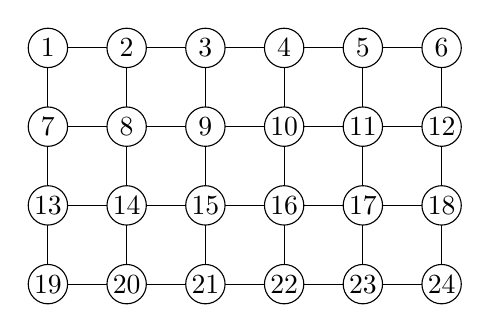
\begin{tikzpicture}
\draw (0,0) grid (5,3);
\node[draw,circle,minimum size=0.5cm,inner sep=0pt, fill=white, text=black] at (0,3) {$1$};
\node[draw,circle,minimum size=0.5cm,inner sep=0pt, fill=white, text=black] at (1,3) {$2$};
\node[draw,circle,minimum size=0.5cm,inner sep=0pt, fill=white, text=black] at (2,3) {$3$};
\node[draw,circle,minimum size=0.5cm,inner sep=0pt, fill=white, text=black] at (3,3) {$4$};
\node[draw,circle,minimum size=0.5cm,inner sep=0pt, fill=white, text=black] at (4,3) {$5$};
\node[draw,circle,minimum size=0.5cm,inner sep=0pt, fill=white, text=black] at (5,3) {$6$};
\node[draw,circle,minimum size=0.5cm,inner sep=0pt, fill=white, text=black] at (0,2) {$7$};
\node[draw,circle,minimum size=0.5cm,inner sep=0pt, fill=white, text=black] at (1,2) {$8$};
\node[draw,circle,minimum size=0.5cm,inner sep=0pt, fill=white, text=black] at (2,2) {$9$};
\node[draw,circle,minimum size=0.5cm,inner sep=0pt, fill=white, text=black] at (3,2) {$10$};
\node[draw,circle,minimum size=0.5cm,inner sep=0pt, fill=white, text=black] at (4,2) {$11$};
\node[draw,circle,minimum size=0.5cm,inner sep=0pt, fill=white, text=black] at (5,2) {$12$};
\node[draw,circle,minimum size=0.5cm,inner sep=0pt, fill=white, text=black] at (0,1) {$13$};
\node[draw,circle,minimum size=0.5cm,inner sep=0pt, fill=white, text=black] at (1,1) {$14$};
\node[draw,circle,minimum size=0.5cm,inner sep=0pt, fill=white, text=black] at (2,1) {$15$};
\node[draw,circle,minimum size=0.5cm,inner sep=0pt, fill=white, text=black] at (3,1) {$16$};
\node[draw,circle,minimum size=0.5cm,inner sep=0pt, fill=white, text=black] at (4,1) {$17$};
\node[draw,circle,minimum size=0.5cm,inner sep=0pt, fill=white, text=black] at (5,1) {$18$};
\node[draw,circle,minimum size=0.5cm,inner sep=0pt, fill=white, text=black] at (0,0) {$19$};
\node[draw,circle,minimum size=0.5cm,inner sep=0pt, fill=white, text=black] at (1,0) {$20$};
\node[draw,circle,minimum size=0.5cm,inner sep=0pt, fill=white, text=black] at (2,0) {$21$};
\node[draw,circle,minimum size=0.5cm,inner sep=0pt, fill=white, text=black] at (3,0) {$22$};
\node[draw,circle,minimum size=0.5cm,inner sep=0pt, fill=white, text=black] at (4,0) {$23$};
\node[draw,circle,minimum size=0.5cm,inner sep=0pt, fill=white, text=black] at (5,0) {$24$};
\end{tikzpicture}}
\caption{Communication graph: nodes represent agents and links represent available communication among agents.}\label{fig_communication}
\end{figure}
Let the communication graph is given in Fig. 1 and $\textbf{B}_{i,\epsilon_1} = \left[\begin{matrix}\textbf{0}_{5 \times 15} & \textbf{I}_{5}\end{matrix}\right], \forall i \in \{1, 2, \dots, 24\}$. The vector $\textbf{b}_{i,\epsilon_1}$ is chosen randomly.
In addition, we assume that the first $5$ elements in local variable vectors are common variables. In other word, $\textbf{P}_{ij} = \textbf{P}_{ji} = \left[\begin{matrix}\textbf{I}_5 & \textbf{0}_{5 \times 15}\end{matrix}\right]$ for all pairs $(i,j)$ of neighboring agents.
 
We use MATLAB to test the effectiveness of our designed method in finding the least square solution for a hundred numerical examples.
In each example, we choose $\textbf{A}_i \in \mathbb{R}^{20 \times 20}, \textbf{a}_i \in \mathbb{R}^{20}, \forall i \in \{1, 2, \dots, 24\},$ randomly. The ADMM-based solution method (\ref{eq_updatelaw_primal_detailed}-\ref{eq_updatelaw_dual}) is run with the selection of $\rho = 1, \textbf{G}_i = 0.1 \textbf{I}, \forall i,$ and the initial starting point $\textbf{w}_i(0) = \textbf{0}, \forall i$.
\begin{figure}[htb]
\centering
\includegraphics[width=0.5\textwidth]{ADMM_result.png}
\caption{The convergence to the least square solution of the second example. Algorithm 1 requires $370$ iterations (\ref{eq_updatelaw_primal_detailed}-\ref{eq_updatelaw_dual}).}\label{fig_result}
\end{figure}
Fig. \ref{fig_result} shows the simulation results corresponding to two examples having the fastest convergence rate (blue lines) and the slowest convergence rate (red lines). In this figure, the solid lines represent the convergence of the estimated solution in the update (\ref{eq_updatelaw_primal_detailed}-\ref{eq_updatelaw_dual}) to one optimal solution $\textbf{x}^{opt}$ of the problem \eqref{eq_distributed_optADMM}. The dashed lines illustrate to the evolution of the function $|\Psi(s) - \Psi^{opt}|$ where $\Psi(s) = \sum_{i = 1}^{24}\left(\textbf{x}_i(s)^T\textbf{Q}_i\textbf{x}_i(s) + \textbf{q}_i^T\textbf{x}_i(s)\right)$ is the cost function value of the estimated solution at the iteration step $s \ge 0$ and $\Psi^{opt} = \sum_{i = 1}^{24}\left((\textbf{x}_i^{opt})^T\textbf{Q}_i\textbf{x}_i^{opt} + \textbf{q}_i^T\textbf{x}_i^{opt}\right)$ is the optimal cost function value.
From the simulation result, it is easy to verify the asymptotic convergence of the estimated solution to the optimal one. A practical solution can be achieved after about $2000$ iterations. In addition, we measure the computation time required by each agent in every iteration step. The maximum time required by one agent for $2000$ iteration is $0.5$ second.
%%%%%%%%%%%%%%%%%%%%%%%%%%%%%%%%%%%%%%%%%%%%%%%%%%%%%%%%%%%%%%%%%%%%%%%%%%%%%%%%%%%%%%%%%%
\section{Conclusion}
%%%%%%%%%%%%%%%%%%%%%%%%%%%%%%%%%%%%%%%%%%%%%%%%%%%%%%%%%%%%%%%%%%%%%%%%%%%%%%%%%%%%%%%%%%
In this paper, we considered a linear algebraic equation $\textbf{H}\textbf{z} = \textbf{h}$ when rows and columns of the matrix $\textbf{H}$ are dispensed across a network of agents. By introducing some temporary variables, finding the equation's least square solution is reformulated into a distributed optimization problem. Then, we apply a proximal ADMM algorithm to design a distributed solution method for agents to solve the formulated optimization problem cooperatively. 
The convergence of the estimated solution of every agent to its corresponding parts in one exact least square solution of the considered linear algebraic equation is at an exponential rate.
%%%%%%%%%%%%%%%%%%%%%%%%%%%%%%%%%%%%%%%%%%%%%%%%%%%%%%%%%%%%%%%%%%%%%%%%%%%%%%%%%%%%%%%%%%
%\section*{acknowledgement}
%This work was supported by the National Research Foundation of Korea (NRF) grant funded by the Korea government (MSIT) (2019R1A4A1029003).
%%%%%%%%%%%%%%%%%%%%%%%%%%%%%%%%%%%%%%%%%%%%%%%%%%%%%%%%%%%%%%%%%%%%%%%%%%%%%%%%%%%%%%%%%%
\bibliographystyle{IEEEtran}
\bibliography{mylib}
%%%%%%%%%%%%%%%%%%%%%%%%%%%%%%%%%%%%%%%%%%%%%%%%%%%%%%%%%%%%%%%%%%%%%%%%%%%%%%%%%%%%%%%%%%
%%%%%%%%%%%%%%%%%%%%%%%%%%%%%%%%%%%%%%%%%%%%%%%%%%%%%%%%%%%%%%%%%%%%%%%%%%%%%%%%%%%%%%%%%%
\end{document}
